\section{Feature Selection}
\label{sec:featureselection}
Selecting only the most relevant features for the regression model is crucial
because it reduces input noise~\citep{mohri2012foundations}, which in turn
increases the prediction accuracy and reduces overfitting. To do so, we
visually inspect and compare feature distribution of different movies
performance groups ($G_1$, $G_2$, $G_3$) and use statistical dependency
metrics\footnote{Statistical dependency metrics are measures that can be
 calculated from sets of data in order to access information about their
 dependence.}.

First, each feature's correlation with all success parameters (economic success
given by gross, public acceptance given by ratings and movie popularity given
by number of votes) were calculated using the Pearson correlation
coefficient~\citep{pearson}. The correlation levels were \textit{low}, with
absolute values ranging between $0$ and $0.57$ for all features. Then, visual
inspection of the scatter plots confirmed that there is no evident
\textit{linear} relationship among all features and the success parameters.

Therefore, we performed a second analysis with: (\textit{i}) the
\textit{distance correlation}\footnote{Distance correlation is a measure of
statistical dependence between two variables. This measure is zero if and only
if the variables are statistically independent~\citep{szekely2007measuring}.}
to detect the strength of non-linear dependence among variables, and
(\textit{ii}) the \textit{Spearman correlation}, for monotonic
relationships~\citep{spearman1904proof}. Table~\ref{tab:corr_both} shows the
results considering only features derived from \textit{square clustering} and
\textit{neighbor overlap}, in which many features present high degrees of
dependence (other metrics provided similar results). Pearson coefficients were
very similar to Spearman coefficients, but they were also included in the
tables for completeness. Negative numbers for Spearman indicates inversely
related variables.

\begin{table}[t]
\centering
\caption{\label{tab:corr_both}Correlation for different features considering all aggregation metrics and success parameters (V:\@ votes, R:\@ ratings, G:\@ gross). 
}
%%\vspace{.5 cm}
\begin{subtable}[b]{\textwidth}
 \caption{\label{tab:corr_squarec} \textbf{Features generated from square clustering}}
\centering
\begin{tabular}{@{}lrrrrrrrrr@{}}
\toprule
\multirow{2}{*}{Aggregator}
& \multicolumn{3}{@{}c@{}}{Distance Corr.} & \multicolumn{3}{c}{Spearman} & \multicolumn{3}{c}{Pearson} \\
\cmidrule(r){2-4} \cmidrule(l){5-7} \cmidrule(l){8-10}
 & \multicolumn{1}{c}{V} & \multicolumn{1}{c}{R} & \multicolumn{1}{c}{G} &
\multicolumn{1}{c}{V} & \multicolumn{1}{c}{R} & \multicolumn{1}{c}{G} & \multicolumn{1}{c}{V} & \multicolumn{1}{c}{R} & \multicolumn{1}{c}{G}  \\ \midrule
Std. Deviation & $~.24$ & $~.08$ & $~.16$ & $-.23$  & $~.06$  & $-.19$ & $-.23$ & $.07$ & $-.14$ \\
Contraction    & $.17$  & $.10$  & $.08$  & $-.33$  & $.13 $  & $-.13$ & $-.13$ & $.06$ & $-.06$ \\
Maximum        & $.26$  & $.10$  & $.16$  & $-.34$  & $.13 $  & $-.20$ & $-.26$ & $.09$ & $-.15$ \\
Minimum        & $.23$  & $.14$  & $.07$  & $-.37$  & $.19 $  & $-.10$ & $-.15$ & $.08$ & $-.04$ \\
Mean           & $.27$  & $.10$  & $.17$  & $-.38$  & $.15 $  & $-.23$ & $-.26$ & $.09$ & $-.16$ \\
Median         & $.26$  & $.10$  & $.17$  & $-.40$  & $.15 $  & $-.20$ & $-.25$ & $.08$ & $-.16$ \\
Harmonic Mean  & $.26$  & $.13$  & $.12$  & $-.40$  & $.16 $  & $-.23$ & $-.20$ & $.10$ & $-.08$ \\ \bottomrule
\end{tabular}
\end{subtable}

\vspace{6pt}

\begin{subtable}[b]{\textwidth}
 \caption{\label{tab:corr_noverlap} \textbf{Features generated from neighbor overlap}}
\centering
\begin{tabular}{@{}lrrrrrrrrr@{}}
\toprule
\multirow{2}{*}{Aggregator}
& \multicolumn{3}{@{}c@{}}{Distance Corr.} & \multicolumn{3}{c}{Spearman} & \multicolumn{3}{c}{Pearson} \\
\cmidrule(r){2-4} \cmidrule(l){5-7} \cmidrule(l){8-10}
 & \multicolumn{1}{c}{V} & \multicolumn{1}{c}{R} & \multicolumn{1}{c}{G} &
\multicolumn{1}{c}{V} & \multicolumn{1}{c}{R} & \multicolumn{1}{c}{G} & \multicolumn{1}{c}{V} & \multicolumn{1}{c}{R} & \multicolumn{1}{c}{G}  \\ \midrule
Std. Deviation  & $~.09$  & $~.13$  & $~.16$  & $~.04$  & $-.12 $  & $-.17$ & $.06$ & $-.12$ & $-.15$ \\
Maximum        & $.11$  & $.13$  & $.13$  & $.12$  & $-.14 $  & $-.14$ & $.12$ & $-.13$ & $-.13$ \\
Midrange       & $.09$  & $.10$  & $.16$  & $.02$  & $-.08 $  & $-.18$ & $.05$ & $-.80$ & $-.16$ \\
Minimum        & $.21$  & $.09$  & $.15$  & $-.18$  & $.06 $  & $-.14$ & $-.18$ & $.07$ & $-.13$ \\
Mean           & $.19$  & $.06$  & $.25$  & $-.15$  & $.00 $  & $-.25$ & $-.15$ & $.00$ & $-.24$ \\
Median         & $.19$  & $.05$  & $.23$  & $-.13$  & $.01 $  & $-.21$ & $-.17$ & $.02$ & $-.23$ \\
Harmonic Mean  & $.24$  & $.09$  & $.22$  & $-.24$  & $.09 $  & $-.20$ & $-.24$ & $.08$ & $-.21$ \\ \bottomrule
\end{tabular}
\end{subtable}

\end{table}


Based on this preliminary analysis, the features with lowest levels of
dependency with respect to the three success parameter were filtered out.
Cross-validation trials showed that removing such features actually
\textit{improved} model accuracy. Features that did not cause any performance
loss were iteratively removed, until no further feature could be removed.  At
the end of this procedure, only \textbf{23 features remained}. Of those
features, 19 are non-topological: nine genres (romance, comedy, horror,
adventure, thriller, mystery, drama, action, and documentary), three continents
(North America, Europe, Africa), duration time, budget (log transform),
previous success (aggregated by node contraction) given by mean ratings and
mean votes, previous success (aggregated by mean) given by mean gross and mean
votes, and previous experience (aggregated by node contraction) given by number
of past joined productions. The remaining four are topological: degree
(aggregated by node contraction), team size, closeness (aggregated by median)
and clustering (aggregated by harmonic mean). Note that although only 4
topological features were selected for the prediction task, a total of 57
topological features are calculated for each movie (see
Table~\ref{tab:features}).

Further adding any feature to this set, such as more binary features for
genres and continents (or any of the others feature from
Table~\ref{tab:features}), either makes no noticeable effect or impairs the
model's accuracy. An overview of all 23 selected features is presented
Table~\ref{tab:selected_features}.

\bgroup\def\arraystretch{1.2}
\begin{table*}[!t]
\caption{\label{tab:selected_features}Set of features selected to be used in the regression model. The topological features are listed last.} 
\centering
\small
\begin{tabular}{@{}p{2.0cm} p{3.75cm} >{\centering}p{2.9cm}@{} p{5.8cm}@{}}
\toprule
\parbox[t]{1.6cm}{Based on}  & \parbox[t]{3.05cm}{Feature Type} & \parbox[t]{2.9cm}{\# of features} & Description \\
\midrule
Genre               & Binary            & 9                  &  One for each of the genres:
                                                              ``Romance'', ``Comedy'', ``Horror'', ``Adventure'',
                                                              ``Thriller'', ``Mistery'', ``Drama'', ``Action'' and ``Documentary''. \\
Continent           & Binary            & 3                  & Binary features for each of the continents: Africa, Europe, North America. \\
Runtime             & Integer           & 1                  & Movie's runtime in minutes. \\
Budget              & Log Transform     & 1                  & The logarithm of the movie's budget adjusted adjusted to present US Dollars. \\
Previous success    & \parbox[t]{4.1cm}{
                      Ego-metric
                      aggregation:\\
                      node contraction} & 2                  & Mean ratings and mean votes for movies previously
                                                              produced by one or more agents. \\
Previous success    & \parbox[t]{4.1cm}{
                      Ego-metric
                      aggregation:\\
                      mean}              & 2                  & Mean of node's past productions gross and number of votes. \\

Previous experience & \parbox[t]{4.1cm}{
                      Ego-metric
                      aggregation:\\
                      node contraction} & 1                  & Number of production previously made by one or more agents
                                                              from the team. \\

\addlinespace[2.ex]
%\multicolumn{4}{@{}l}{\textit{Topological Features}}   \\
\multicolumn{2}{c}{\textit{Topological Features}}   \\
\addlinespace[2.ex] %\midrule
Degree              & \parbox[t]{4.1cm}{
                     Ego-metric
                     aggregation:\\
                     node contraction}  & 1                  & Number of distinct peers from nodes, disregarding nodes in the
                                                              team being analyzed. \\
                                                              team being analyzed. \\
Team Size           & Simple Feature    & 1                  & Number of nodes in the current team. \\
Closeness           & \parbox[t]{4.1cm}{
                      Ego-metric
                      aggregation:\\
                      median}           & 1                  & Median of closeness metric for nodes in the team. \\
Clustering          & \parbox[t]{4.1cm}{
                      Ego-metric
                      aggregation:\\
                      harmonic mean}    & 1                  & Harmonic mean of clustering coefficient for nodes in the team.\\
\bottomrule
\end{tabular}
\end{table*}
\egroup{}


Further confirming this analysis, a visual representation of how informative a
feature is with respect to movie performance is possible by plotting the
feature's distributions next to the three different movie performance groups.
The more different the shapes and values of the distributions, the more they
provide information that can be used to predict performance. Therefore,
Figures~\ref{fig:hist_feat_top}~and~\ref{fig:hist_feat_ntop} respectively show
different distributions for informative topological and non-topological
features.  Both figures confirm the presented features provide useful
information.

\clearpage

\begin{figure}[H]\begin{center}
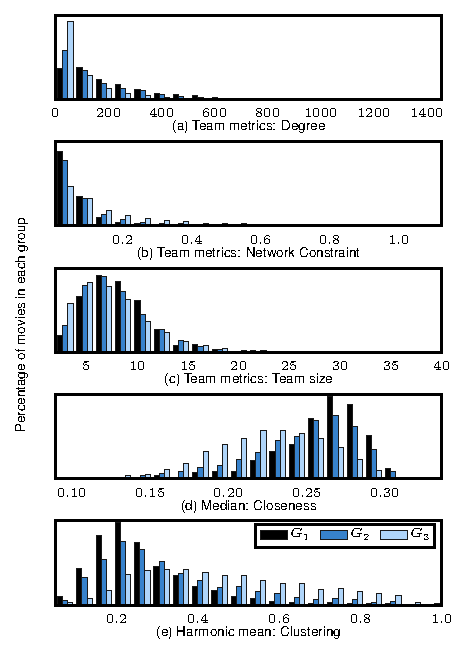
\includegraphics[width=0.78\columnwidth]{../../images/features_hist_top.pdf}
\caption{\label{fig:hist_feat_top}Distribution of topological features for
movies in the three different performance groups. The $x$ axis represents the
portion of movies from the given group (encoded by color) having the specified
value.}
\end{center}\end{figure}


\begin{figure}[H]\begin{center}
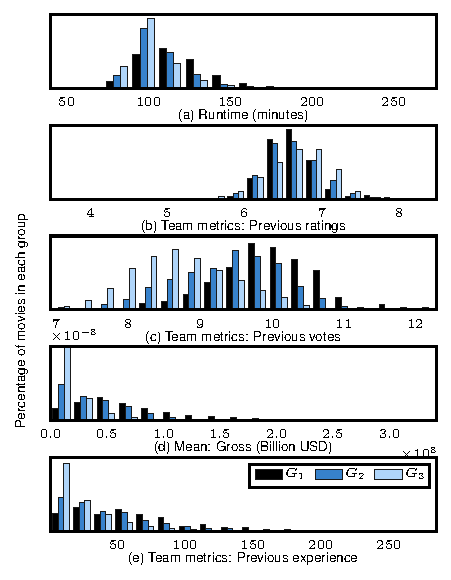
\includegraphics[width=0.78\columnwidth]{../../images/features_hist_ntop.pdf}
\caption{\label{fig:hist_feat_ntop}Distribution of non topological features for
movies in the three different performance groups. The $x$ axis represents the
portion of movies from the given group (encoded by color) having the specified
value.}
\end{center}\end{figure}

\subsection{Producing Successful Movies}
\label{sec:future}
In this section, we assume new teams showing topological characteristics
previously associated to successful movies have a higher probability of
producing successful movies. Under this assumption, we present how our findings
can help to chose agents for a new movie producing team, such that it has
improved success odds.

Figures~\ref{fig:hist_feat_top}~and~\ref{fig:hist_feat_ntop} show movies that
perform better are well determined by their features ranges.  We believe new
teams whose characteristics fall in the same range of values as other
successful teams would be more likely to succeed as well. For example, from
Figure~\ref{fig:hist_feat_top}, movies from the $G_1$ group (blockbusters) are
more likely to have a low clustering coefficient (0--0.3 interval) when
compared to $G_2$ and $G_3$. Moreover, successful teams are likely to have
degree larger than 100, network constraints smaller than 0.1, team sizes of
6--10 people, and closeness greater than 0.25.

We observe that teams with a combined past
experience of 50+ movies are more likely to produce highly successful movies.
Also, teams whose previous movies got an average mean gross of USD 50 million
have a higher chance of producing successful movies. We also see that the mean
rating from movies produced by team members should not deviate much from the
global mean (6--7). Ideally, one should pick producers whose previous
movies received in average about $8,000$ votes.
